% ============================================================================
% Poster: Evaluacion Sistematica de la Precision Estructural de AlphaFold2
% Autor: Jose Antonio Tapia Godinez - ITAM
% Tamano: A1 portrait (594 x 841 mm)
% ============================================================================

\documentclass[20pt,a1paper,portrait]{tikzposter}

% --- Paquetes ---
\usepackage[utf8]{inputenc}
\usepackage[T1]{fontenc}
\usepackage[spanish]{babel}
\usepackage{amsmath, amssymb}
\usepackage{graphicx}
\usepackage{booktabs}
\usepackage{siunitx}
\usepackage{enumitem}
\usepackage{xcolor}
\usepackage{lmodern}

% --- Ruta de figuras ---
\graphicspath{{../reports/latex/figures/}}

% --- Configuracion de siunitx ---
\sisetup{
    output-decimal-marker={,},
    group-separator={.},
    group-minimum-digits=4
}

% --- Tema del poster ---
\usetheme{Default}

% --- Colores ITAM ---
\definecolor{itamblue}{RGB}{0, 54, 99}
\definecolor{itamdark}{RGB}{0, 32, 63}
\definecolor{itamlight}{RGB}{218, 231, 245}
\definecolor{itamaccent}{RGB}{175, 54, 44}
\definecolor{itamgreen}{RGB}{0, 109, 86}
\definecolor{blockbg}{RGB}{247, 250, 253}
\definecolor{paperwarm}{RGB}{253, 254, 252}

\definecolorstyle{ITAM}{
    \definecolor{colorOne}{named}{itamblue}
    \definecolor{colorTwo}{named}{itamdark}
    \definecolor{colorThree}{named}{itamlight}
}{
    \colorlet{backgroundcolor}{paperwarm}
    \colorlet{framecolor}{itamblue}
    % Title - fondo blanco para que el logo ITAM (verde) sea visible
    \colorlet{titlefgcolor}{itamdark}
    \colorlet{titlebgcolor}{white}
    % Block
    \colorlet{blocktitlebgcolor}{itamblue}
    \colorlet{blocktitlefgcolor}{white}
    \colorlet{blockbodybgcolor}{blockbg}
    \colorlet{blockbodyfgcolor}{black}
    % Inner block
    \colorlet{innerblocktitlebgcolor}{itamlight}
    \colorlet{innerblocktitlefgcolor}{itamdark}
    \colorlet{innerblockbodybgcolor}{white}
    \colorlet{innerblockbodyfgcolor}{black}
    % Notes
    \colorlet{notefgcolor}{black}
    \colorlet{notebgcolor}{itamlight}
    \colorlet{noteframecolor}{itamblue}
}

\usecolorstyle{ITAM}
\usetitlestyle[
    width=575mm,
    roundedcorners=10,
    linewidth=2.5pt,
    innersep=6mm,
    titletotopverticalspace=6mm,
    titletoblockverticalspace=7mm
]{Default}
\useblockstyle[
    roundedcorners=10,
    linewidth=2.2pt,
    titleinnersep=5.5mm,
    bodyinnersep=6.5mm
]{Default}
\useinnerblockstyle[
    roundedcorners=8,
    linewidth=1.4pt,
    titleinnersep=5pt,
    bodyinnersep=8pt
]{Default}
\tikzposterlatexaffectionproofoff
\setlist{leftmargin=1.05em, itemsep=0em, topsep=0.05em, parsep=0pt}
\setlength{\parskip}{0.15em}
\emergencystretch=1.5em
\makeatletter
\setlength{\TP@blockverticalspace}{6mm}
\makeatother

% --- Titulo ---
\title{Evaluaci\'on Sistem\'atica de la Precisi\'on Estructural de AlphaFold2}
\newcommand{\postersubtitle}{Validaci\'on PDB--AlphaFold2 con mapeo SIFTS, RMSD estratificado e inferencia bayesiana}

\author{%
    \textbf{Jos\'e Antonio Tapia God\'inez}\textsuperscript{1} \quad
    \textbf{Dr.\ Edgar Francisco Rom\'an Rangel}\textsuperscript{1} (Asesor)
}

\institute{%
    \textsuperscript{1}ITAM, Maestr\'ia en Ciencia de Datos
    \quad --- \quad jose.tapia@itam.mx
}

\titlegraphic{}

\makeatletter
\renewcommand{\TP@maketitle}{%
\centering
\begin{minipage}[c]{0.14\linewidth}
    \centering
    
\includegraphics[height=1.9cm]{logo_itam.pdf}
\end{minipage}%
\hfill
\begin{minipage}[c]{0.82\linewidth}
    \raggedright
    {\color{itamdark}\bfseries\LARGE \@title\par}
    \vspace{0.2em}
    {\color{itamaccent}\large \postersubtitle\par}
    \vspace{0.35em}
    {\normalsize \@author\par}
    {\small \@institute}
\end{minipage}
}
\makeatother

\begin{document}

\maketitle

% ============================================================================
% Tres columnas continuas: evita repeticiones visuales y cortes al final.
% ============================================================================
\begin{columns}

\column{0.32}

\block{1. Motivaci\'on y control SIFTS}{
    \textbf{AlphaFold2} (DeepMind, 2021) predice la estructura 3D de prote\'inas
    a partir de su secuencia de amino\'acidos (GDT 92,4/100 en CASP14).

    \vspace{0.1em}
    \textbf{Pregunta:} \textit{\textquestiondown}cu\'ando puede usarse una predicci\'on de
    AlphaFold2 como sustituto estructural confiable?

    \begin{itemize}
        \item Validaci\'on a gran escala contra estructuras PDB.
        \item Comparaci\'on por longitud, amino\'acido, grupo funcional y elemento.
        \item Base reproducible para comparar con modelos posteriores.
    \end{itemize}

    \vspace{0.1em}
    \textbf{SIFTS} (\textit{Structure Integration with Function, Taxonomy and Sequence}):
    mapea residuos PDB a UniProt, corrigiendo cadena y numeraci\'on.

    \vspace{0.1em}
    \textbf{Control cr\'itico:} sin SIFTS, el RMSD se infla \textbf{35$\times$}.

    \vspace{0.1em}
    \begin{center}
    {\footnotesize
    \begin{tabular}{@{}lcc@{}}
        \toprule
        \textbf{M\'etrica} & \textbf{Sin SIFTS} & \textbf{Con SIFTS} \\
        \midrule
        RMSD mediana & 22,54\,\AA & \textbf{0,64\,\AA} \\
        $<$ 2\,\AA & 13,9\% & \textbf{87,7\%} \\
        $>$ 10\,\AA & 80,9\% & \textbf{0,4\%} \\
        \bottomrule
    \end{tabular}
    }
    \end{center}
}

\block{2. Conjunto de datos}{
    \textbf{10.432 prote\'inas \'unicas} (1 PDB por UniProt ID),
    del archivo SIFTS (68.591 IDs disponibles).

    \vspace{0.1em}
    \begin{center}
    {\footnotesize
    \begin{tabular}{@{}lr@{}}
        \toprule
        \textbf{Etapa} & \textbf{N} \\
        \midrule
        Pares candidatos (SIFTS) & 13.000 \\
        Ambos archivos descargados & 11.384 \\
        Procesados exitosamente & \textbf{10.432} \\
        Tasa de \'exito & 91,6\% \\
        \bottomrule
    \end{tabular}
    }
    \end{center}

    \vspace{0.05em}
    \begin{center}
        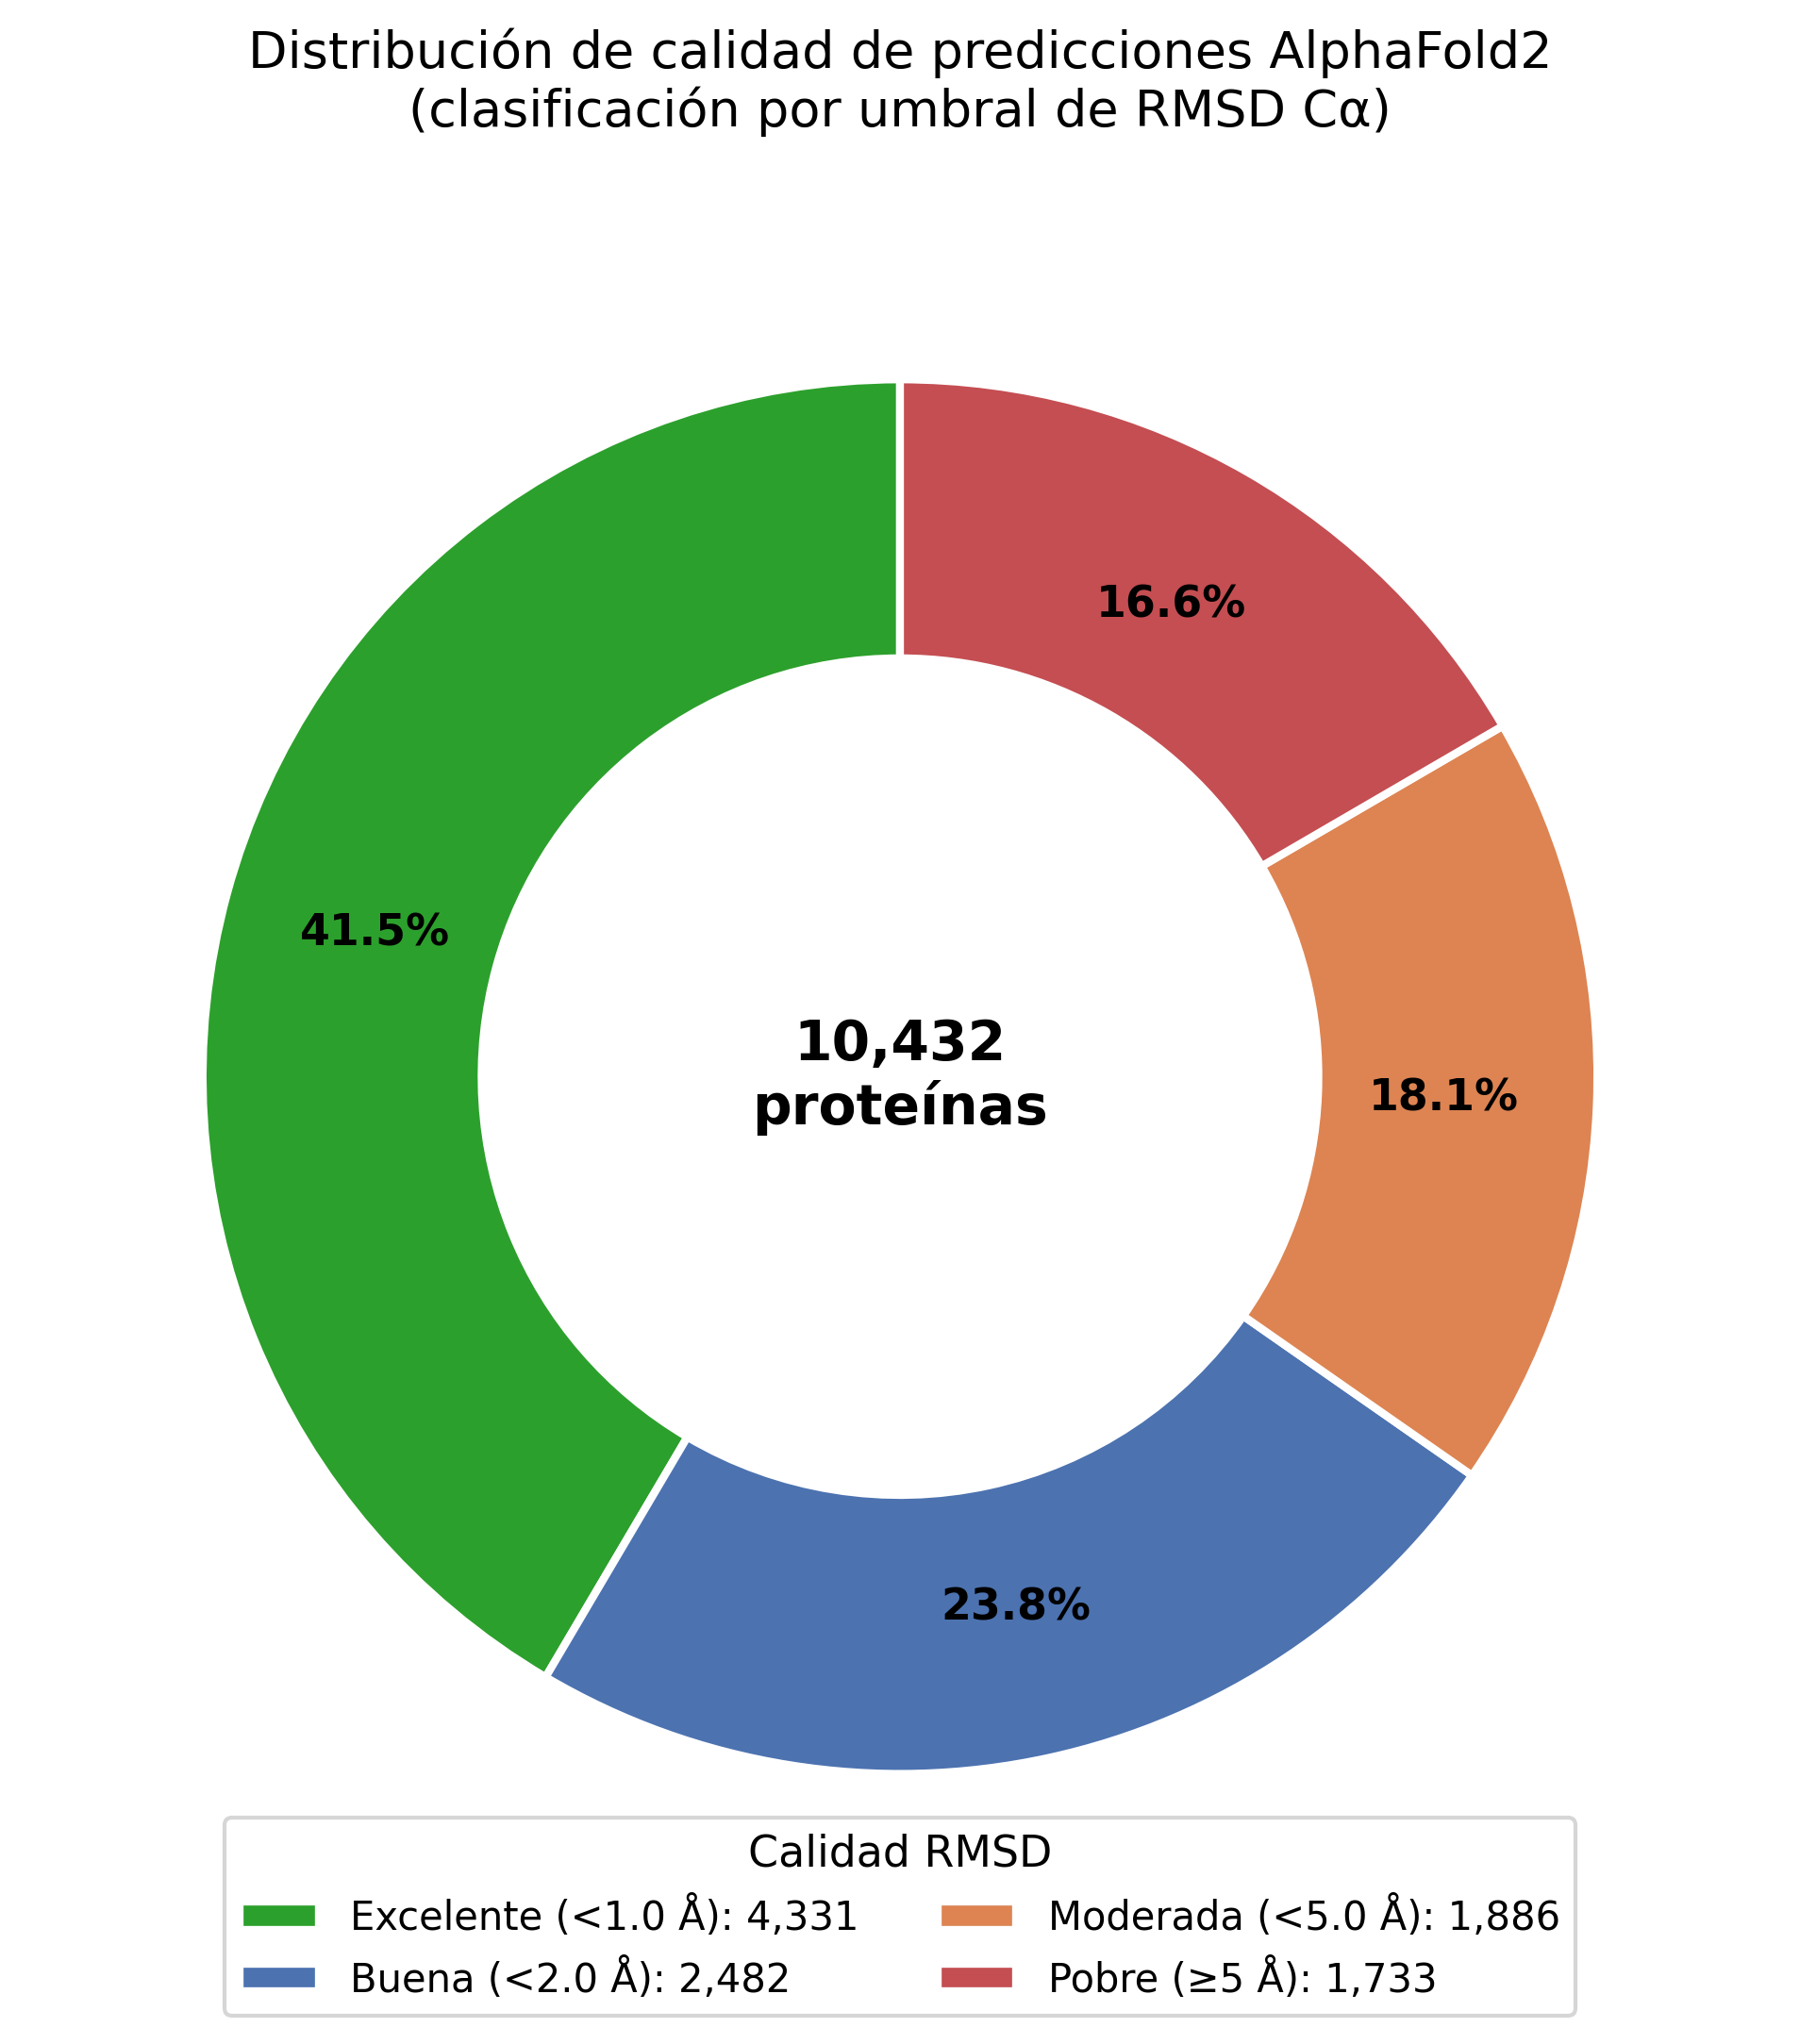
\includegraphics[width=0.72\linewidth]{fig_06g_quality_donut.png}
    \end{center}
    \vspace{-0.7em}
    \begin{center}
        {\footnotesize \textbf{65,3\%} con RMSD $< 2$\,\AA{} (Buena + Excelente)}
    \end{center}
}

\column{0.36}

\block{3. \textit{Pipeline} de evaluaci\'on}{
    \begin{center}
        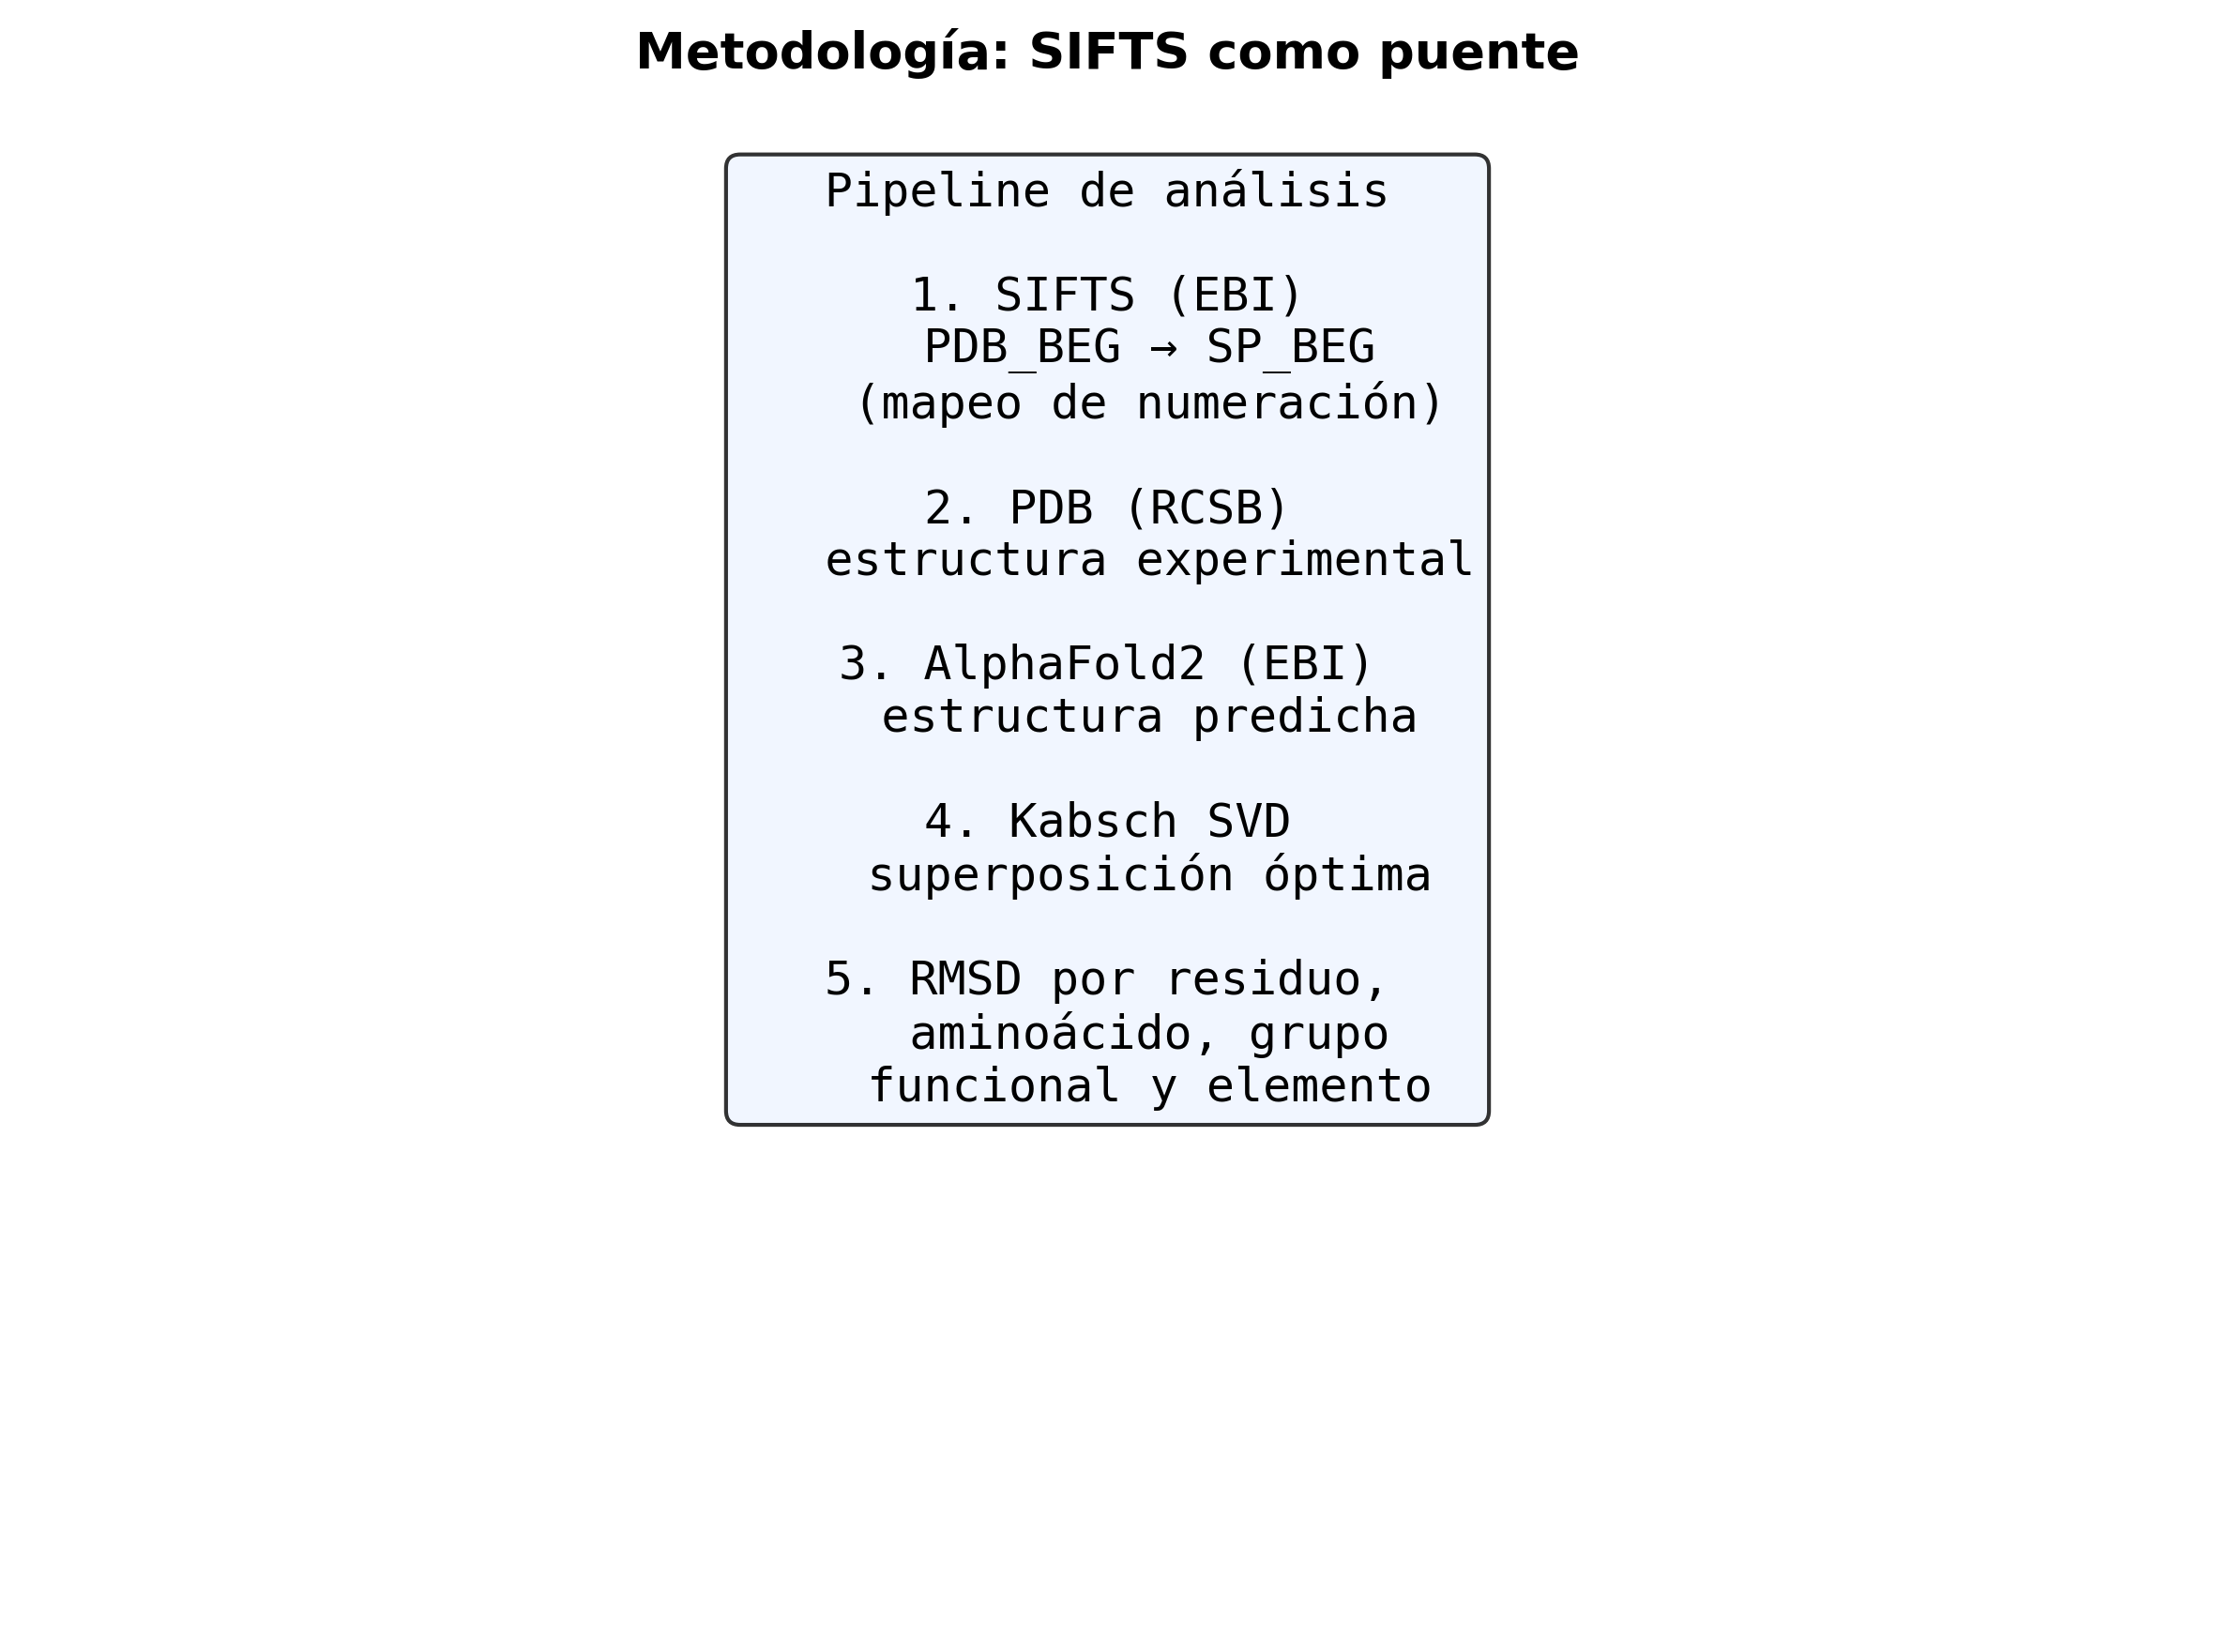
\includegraphics[width=0.72\linewidth]{fig_00a_pipeline.png}
    \end{center}
    \vspace{-0.3em}
    \begin{enumerate}
        \item \textbf{Mapeo SIFTS:} PDB $\to$ UniProt $\to$ AlphaFold.
        \item \textbf{Superposici\'on:} Kabsch (SVD) sobre \'atomos \textit{backbone}.
        \item \textbf{Estratificaci\'on:} longitud $\to$ amino\'acido $\to$ grupo $\to$ elemento.
    \end{enumerate}

    \vspace{0.1em}
    \innerblock{\textbf{M\'etrica principal}}{
        \vspace{-0.7em}
        \begin{equation*}
            \text{RMSD} = \sqrt{\frac{1}{n} \sum_{i=1}^{n} \left\| \mathbf{r}_i^{\,\text{exp}} - \mathbf{r}_i^{\,\text{pred}} \right\|^2}
        \end{equation*}
        \vspace{-0.8em}

        {\footnotesize $<1$\,\AA{} excelente $|$ $<2$\,\AA{} buena $|$ $<5$\,\AA{} moderada $|$ $\geq5$\,\AA{} pobre}
    }
}

\block{4. Resultados globales y longitud}{
    \begin{minipage}[t]{0.48\linewidth}
        \begin{center}
            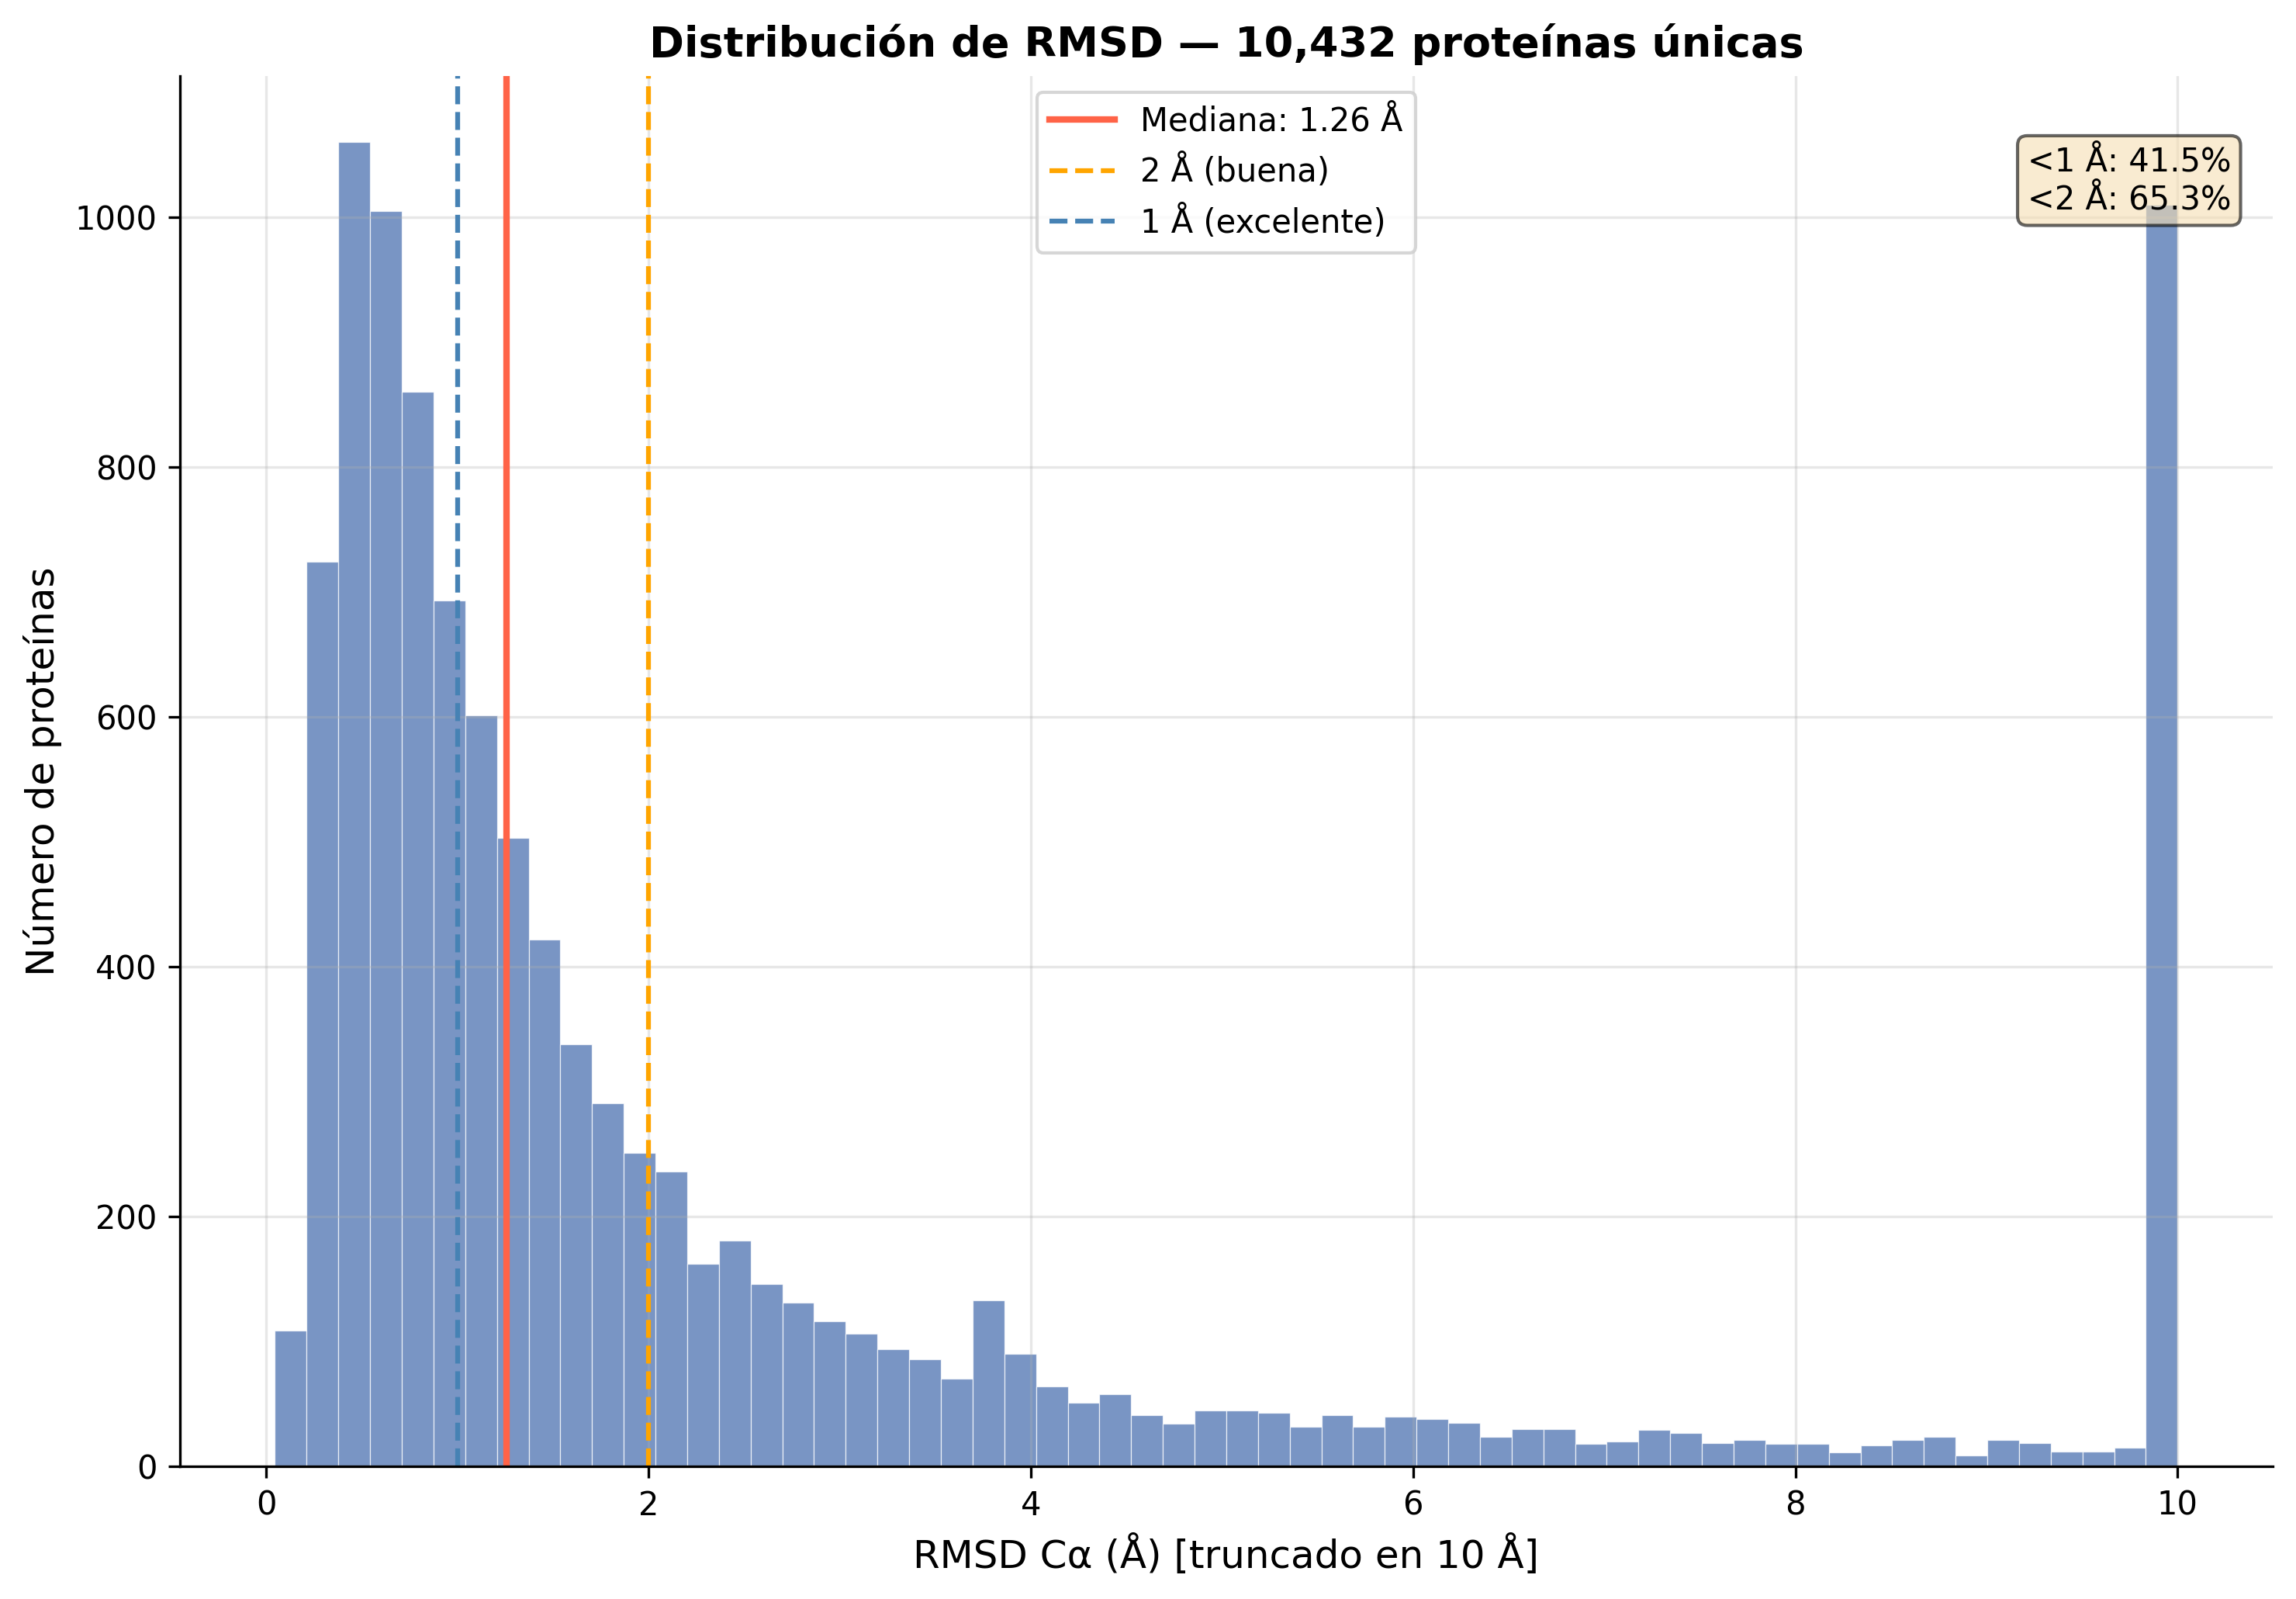
\includegraphics[width=\linewidth]{fig_00c_rmsd_histogram.png}
            \\[-0.4em]
            {\scriptsize Distribuci\'on global RMSD (10.432 prot.)}
        \end{center}
    \end{minipage}%
    \hfill
    \begin{minipage}[t]{0.48\linewidth}
        \begin{center}
            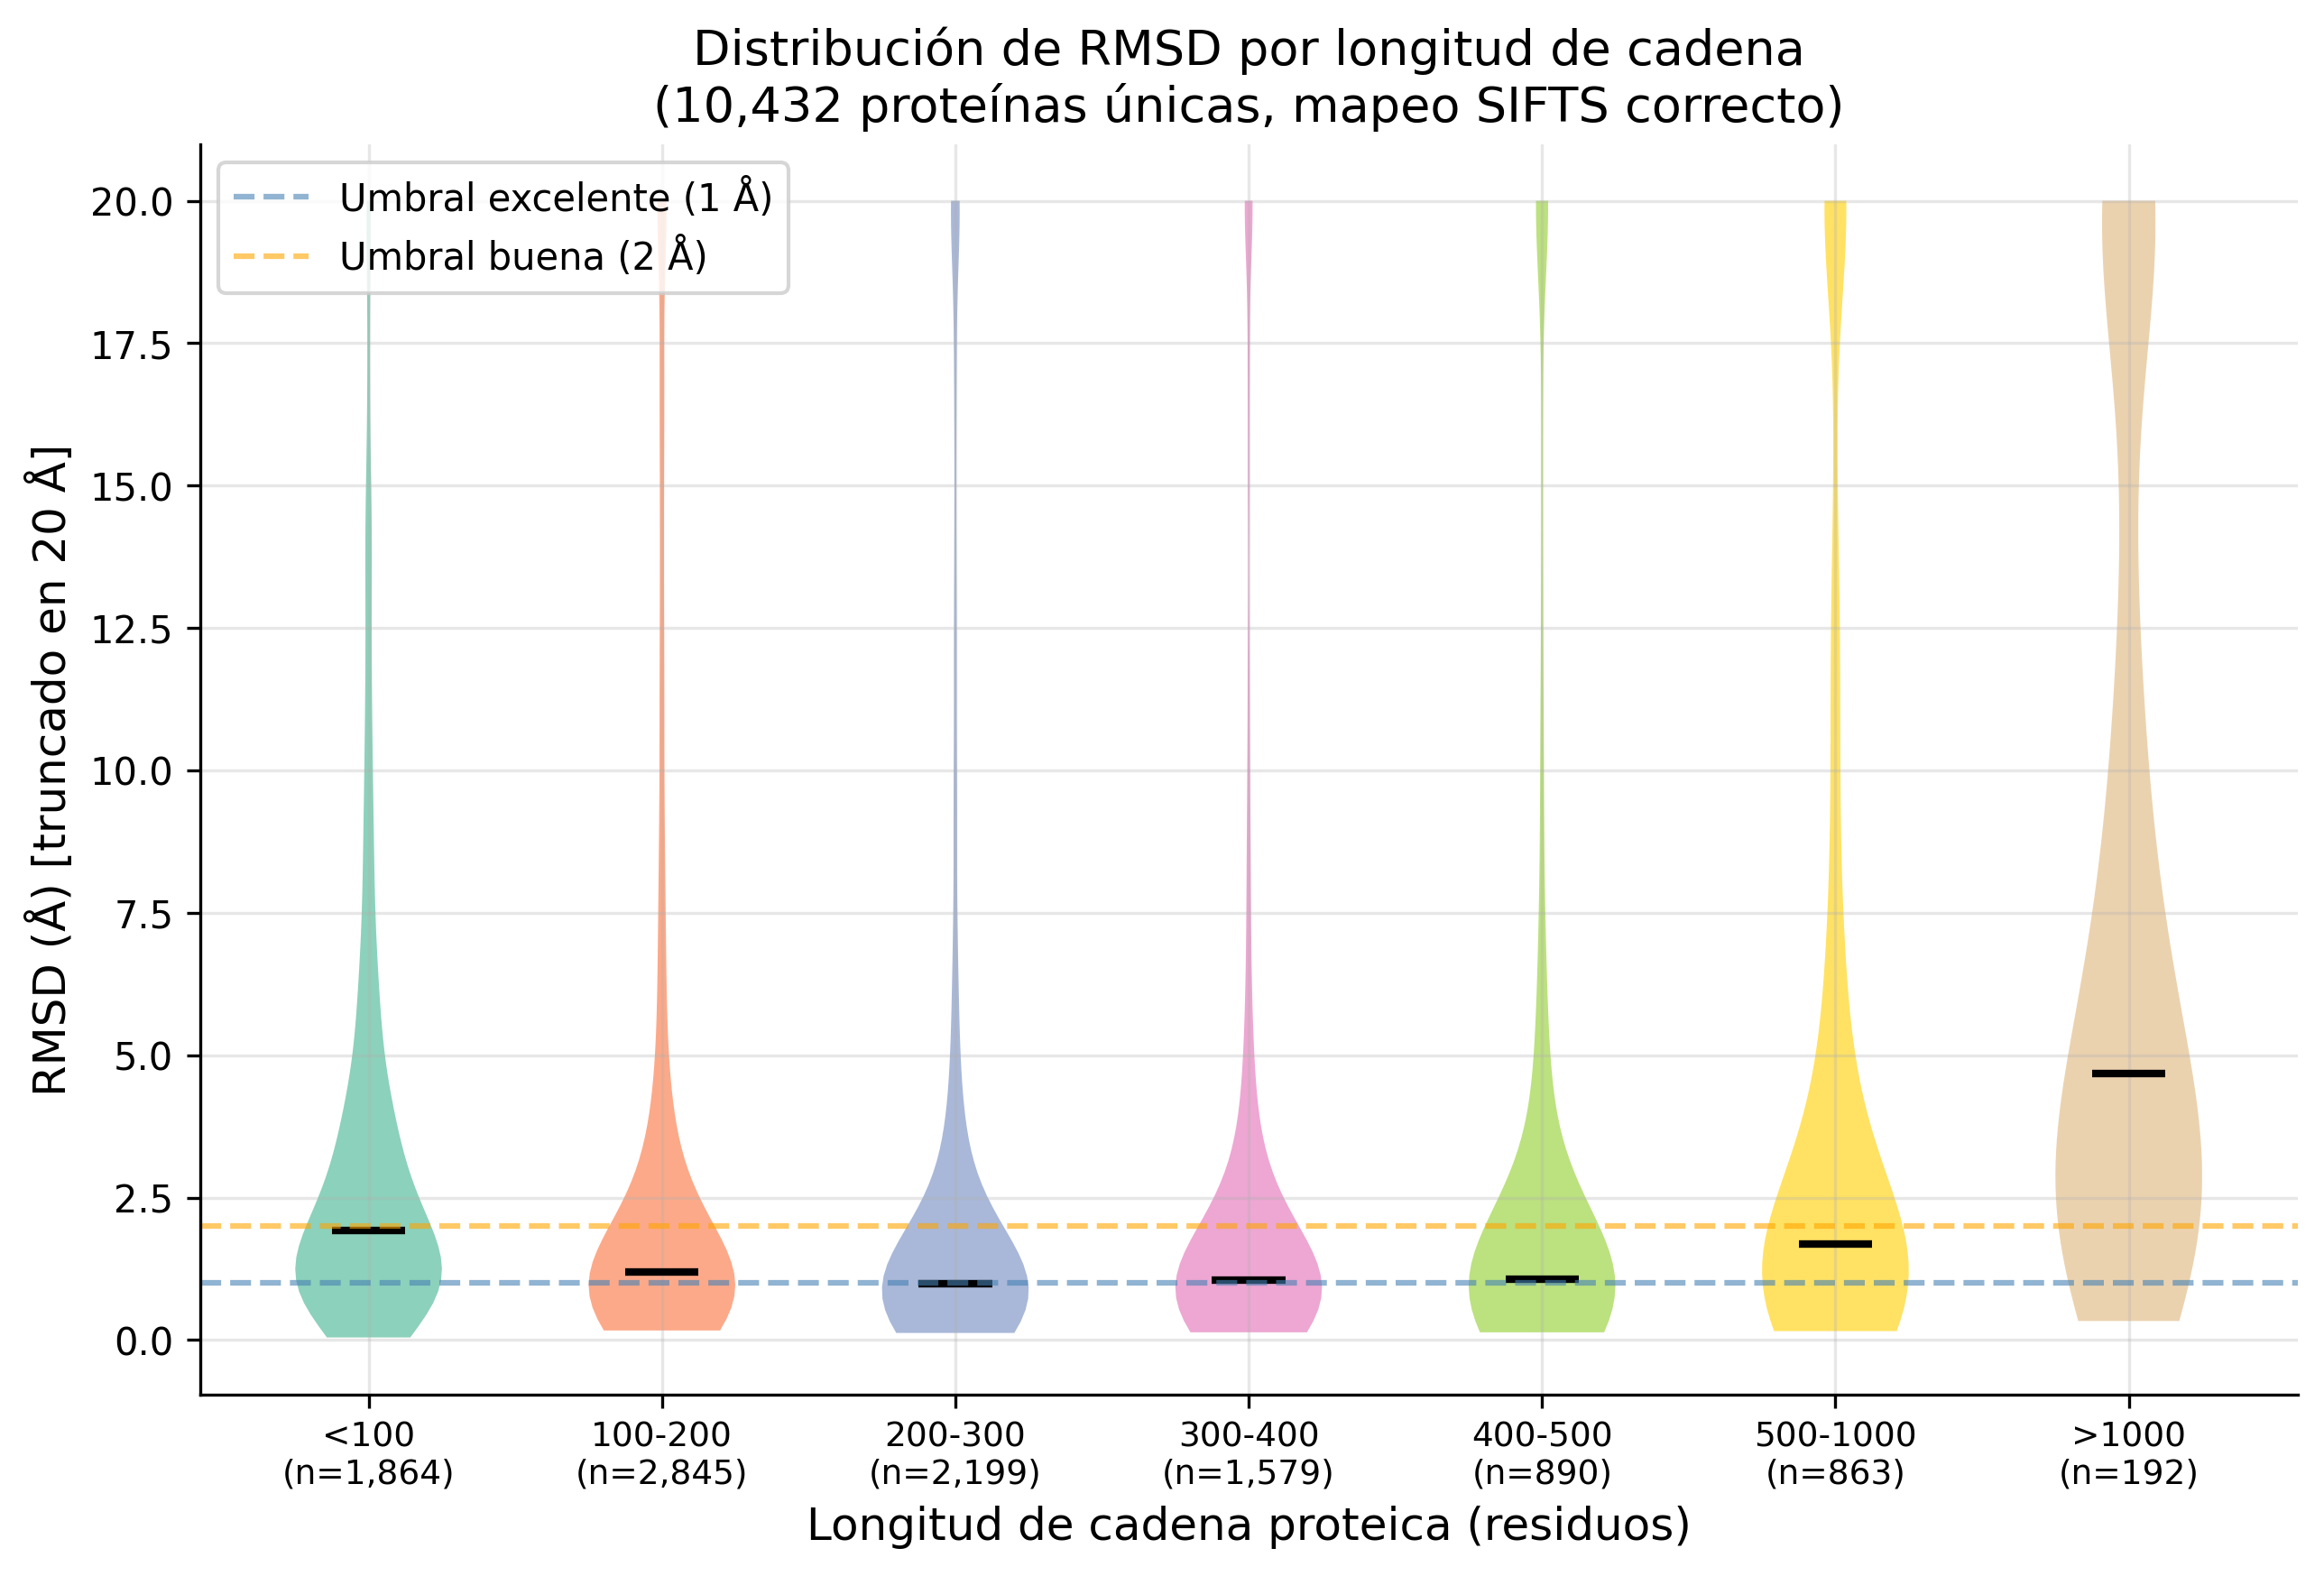
\includegraphics[width=\linewidth]{fig_01_length_violin.png}
            \\[-0.4em]
            {\scriptsize RMSD por categor\'ia de longitud}
        \end{center}
    \end{minipage}

    \vspace{0.05em}
    \begin{center}
    {\footnotesize
    \begin{tabular}{@{}lrcccc@{}}
        \toprule
        \textbf{Categor\'ia} & \textbf{N} & \textbf{Media} & \textbf{Med.} & \textbf{$<$1\,\AA} & \textbf{$<$2\,\AA} \\
        \midrule
        $<$100    & 1.908 & 3,52  & 1,91 & 26,9\% & 52,0\% \\
        100--200  & 2.819 & 3,42  & 1,20 & 43,1\% & 66,9\% \\
        \textbf{200--300} & \textbf{2.194} & \textbf{2,88} & \textbf{0,98} & \textbf{51,1\%} & \textbf{74,0\%} \\
        300--500  & 2.463 & 3,00  & 1,06 & 47,6\% & 73,0\% \\
        500--1000 &   857 & 5,97  & 1,69 & 34,8\% & 55,0\% \\
        $>$1000   &   191 & 10,59 & 4,68 & 5,2\%  & 22,5\% \\
        \midrule
        \textbf{Global} & \textbf{10.432} & \textbf{3,56} & \textbf{1,26} & \textbf{41,5\%} & \textbf{65,3\%} \\
        \bottomrule
    \end{tabular}
    }
    \end{center}

    \vspace{0.05em}
    {\footnotesize \textbf{No existe ``\textit{sweet spot}''}: precisi\'on alta para 100--500 res.
    El \'optimo aparente en 250--300 era un \textbf{artefacto del desfase de numeraci\'on}.}
}

\block{Interpretaci\'on estad\'istica}{
    \begin{itemize}
        \item La \textbf{mediana} describe mejor el desempe\~no t\'ipico que la media,
        porque la distribuci\'on de RMSD tiene cola derecha.
        \item El umbral \textbf{$<2$\,\AA} separa modelos adecuados para uso estructural
        exploratorio de casos que requieren revisi\'on.
        \item Prote\'inas muy largas acumulan incertidumbre por dominios m\'ultiples,
        flexibilidad y diferencias de estado conformacional.
        \item Los \textit{outliers} no son solo ruido: pueden indicar complejos, ligandos,
        dominios ausentes o cambios apo--holo.
    \end{itemize}
}

\column{0.32}

\block{5. Jerarqu\'ia qu\'imica de precisi\'on}{
    \begin{minipage}[t]{0.48\linewidth}
        \begin{center}
            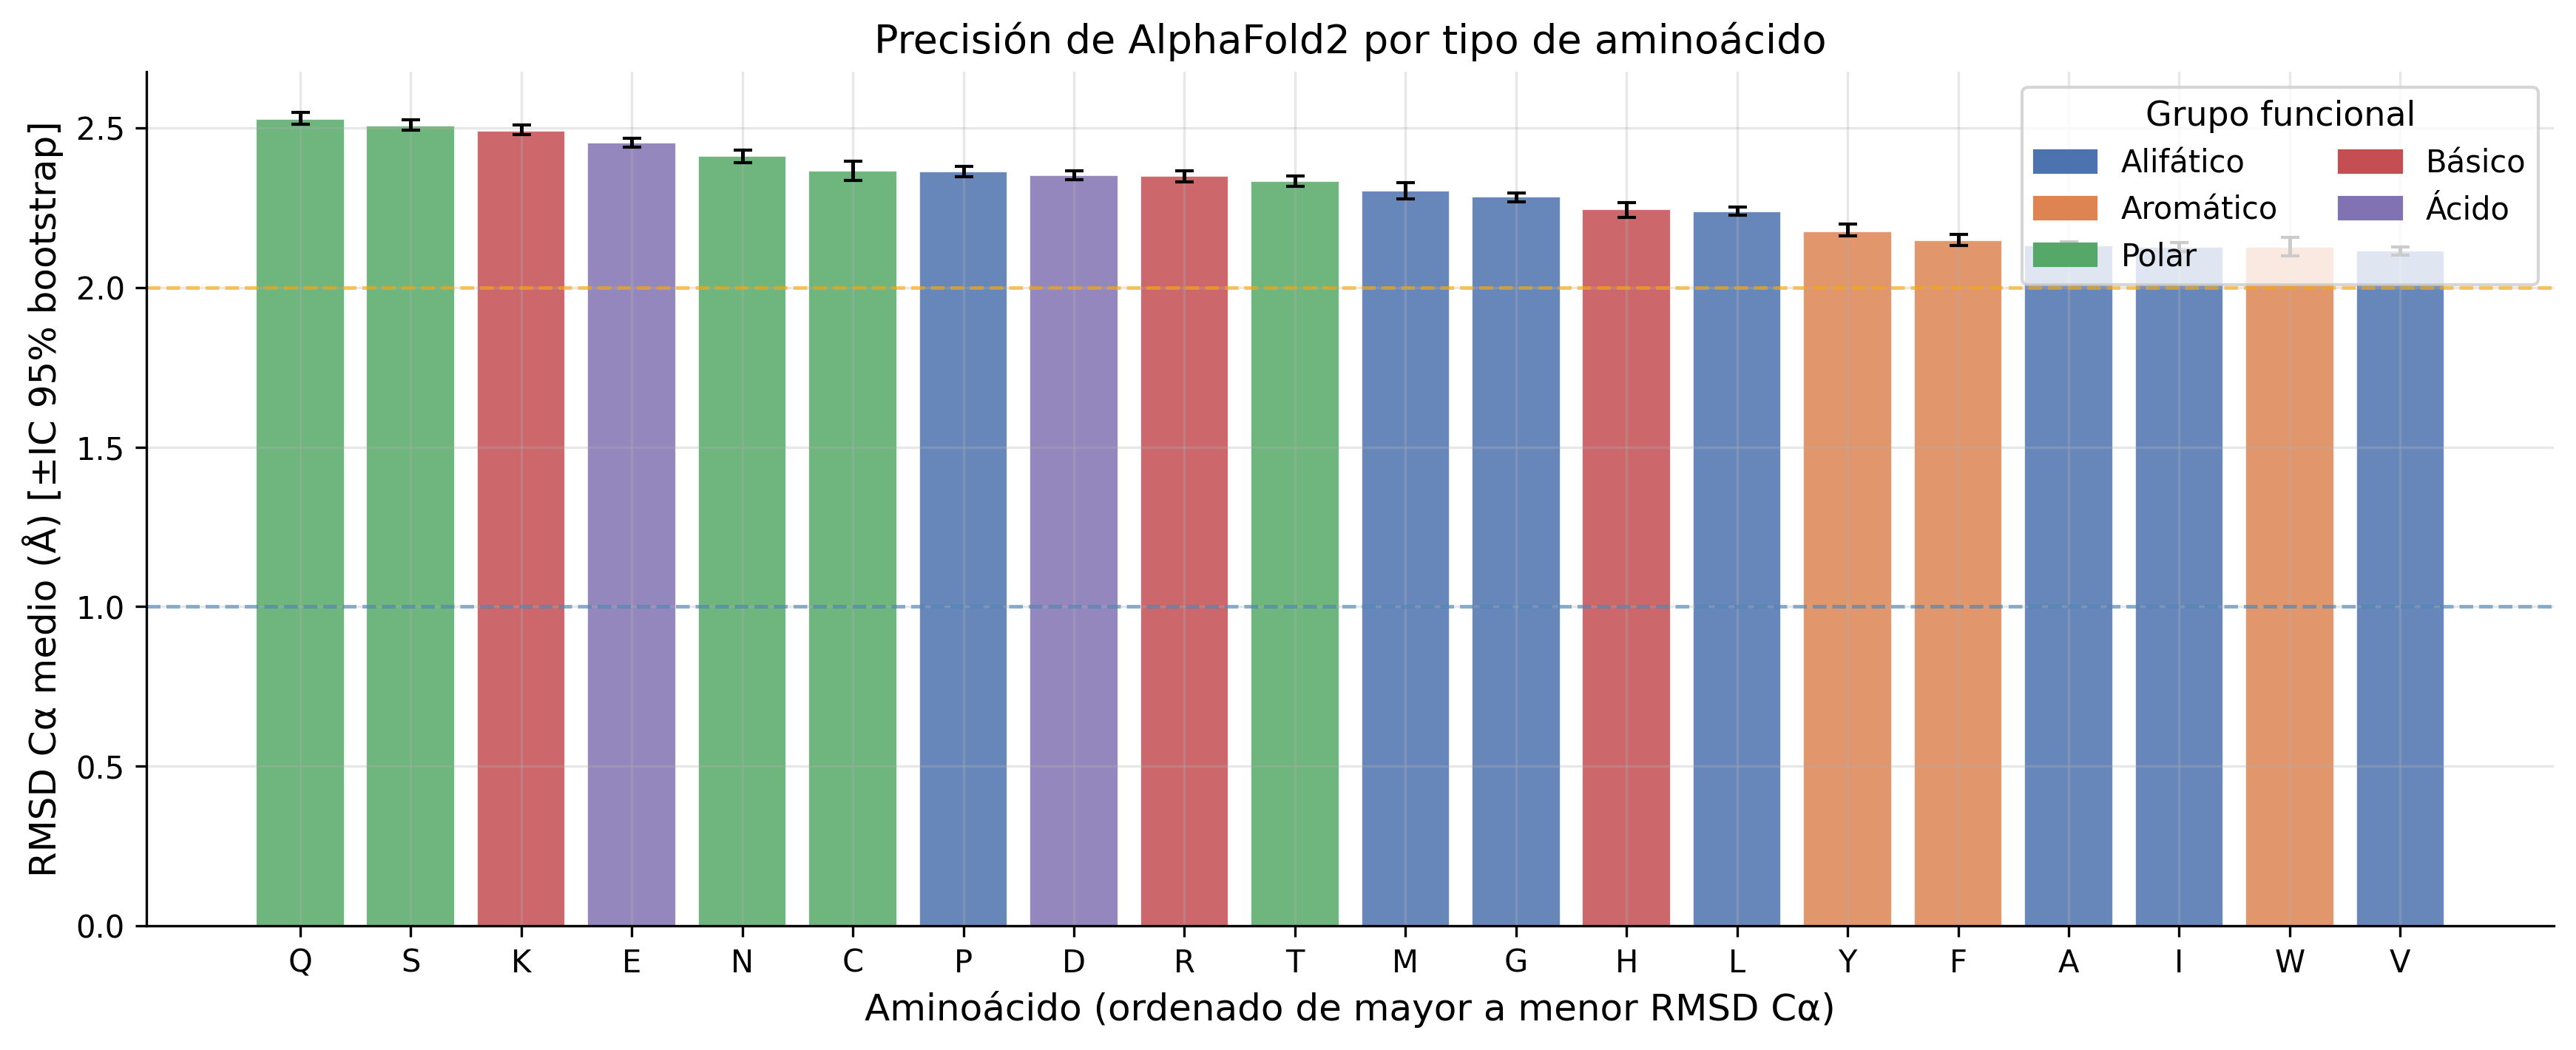
\includegraphics[width=\linewidth]{fig_02_aa_rmsd_sorted.png}
            \\[-0.4em]
            {\scriptsize \textbf{Nivel 2:} RMSD por amino\'acido (2,86M res.)}
        \end{center}
    \end{minipage}%
    \hfill
    \begin{minipage}[t]{0.48\linewidth}
        \begin{center}
            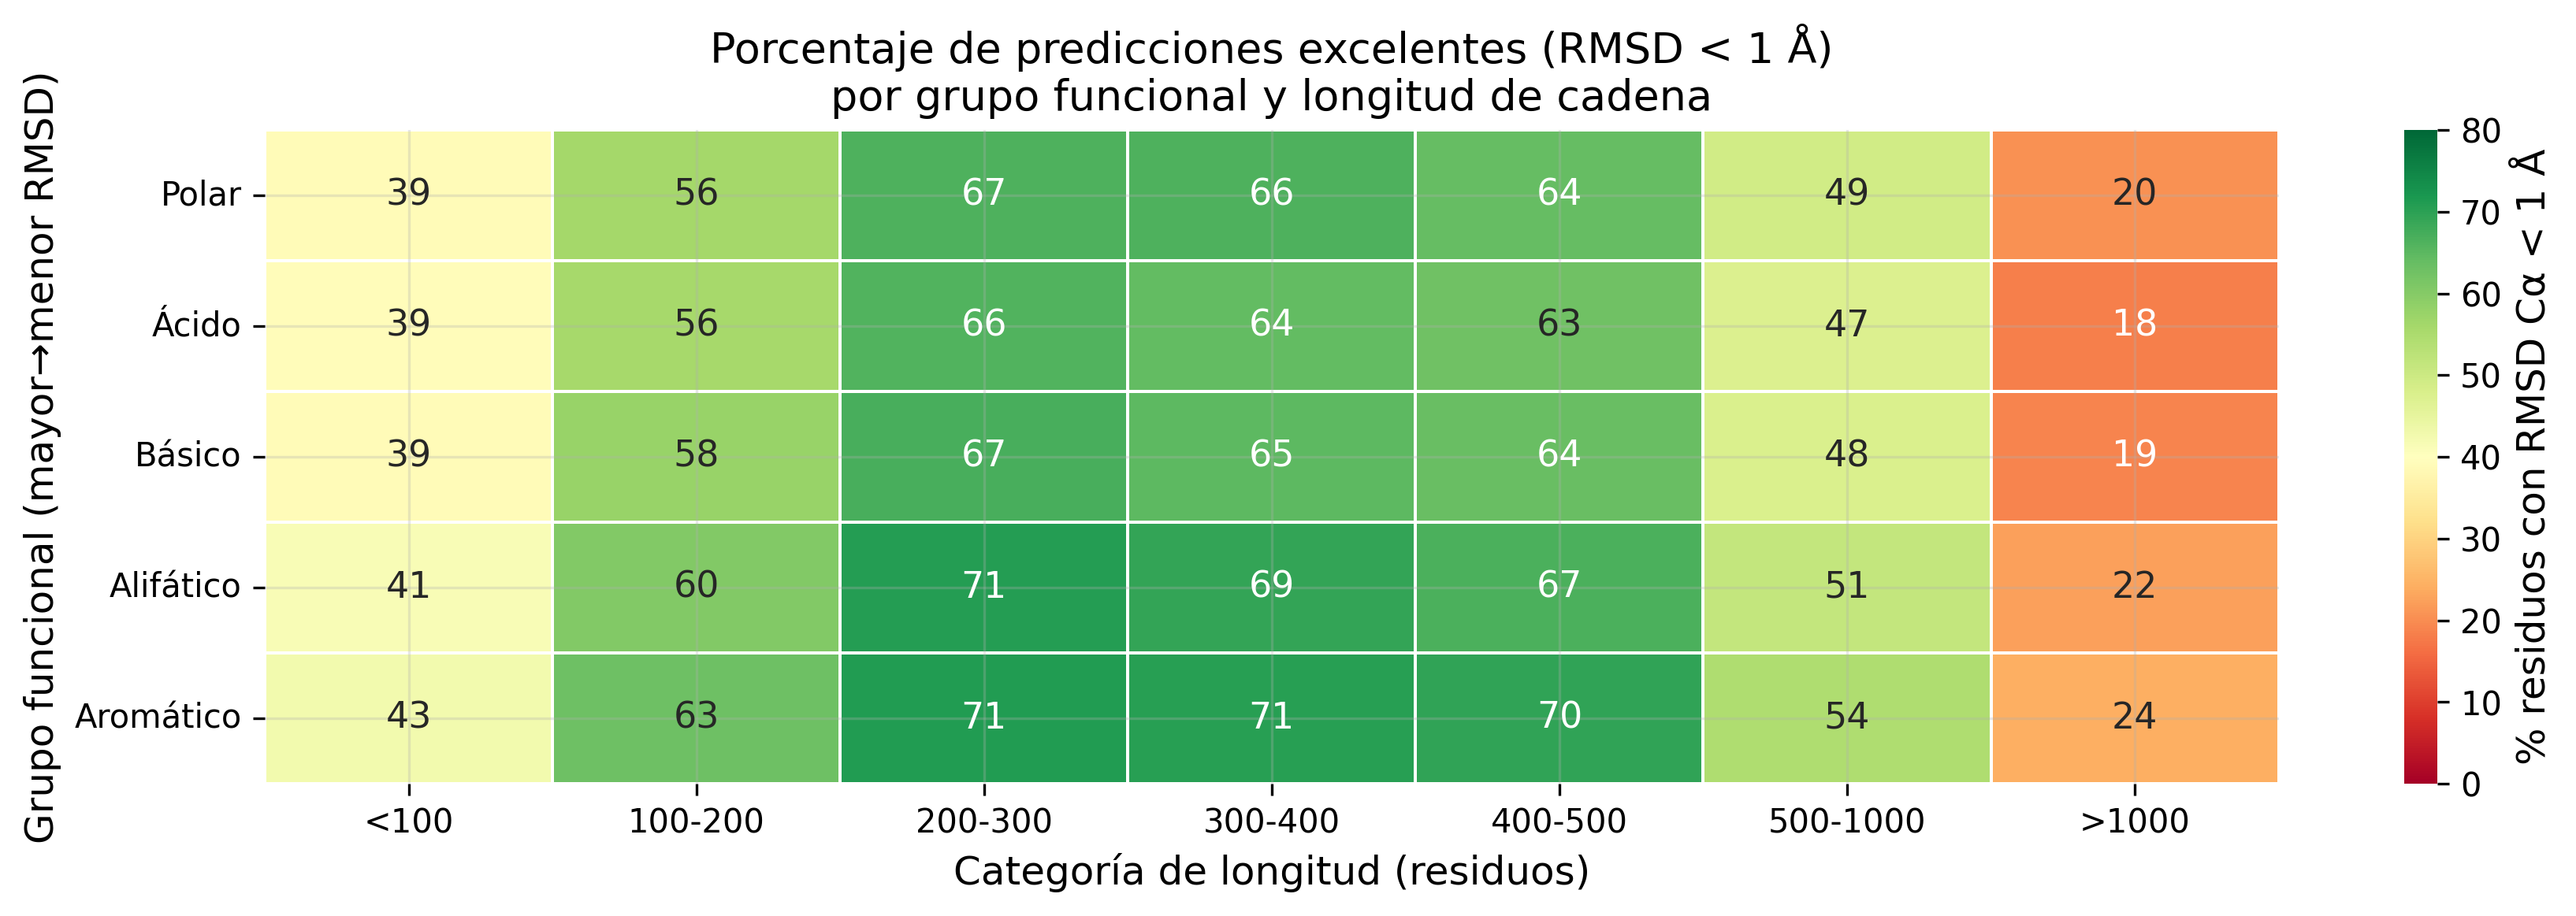
\includegraphics[width=\linewidth]{fig_03_fg_heatmap.png}
            \\[-0.4em]
            {\scriptsize \textbf{Nivel 3:} \% excelente grupo funcional $\times$ longitud}
        \end{center}
    \end{minipage}

    \vspace{0.05em}

    \begin{center}
        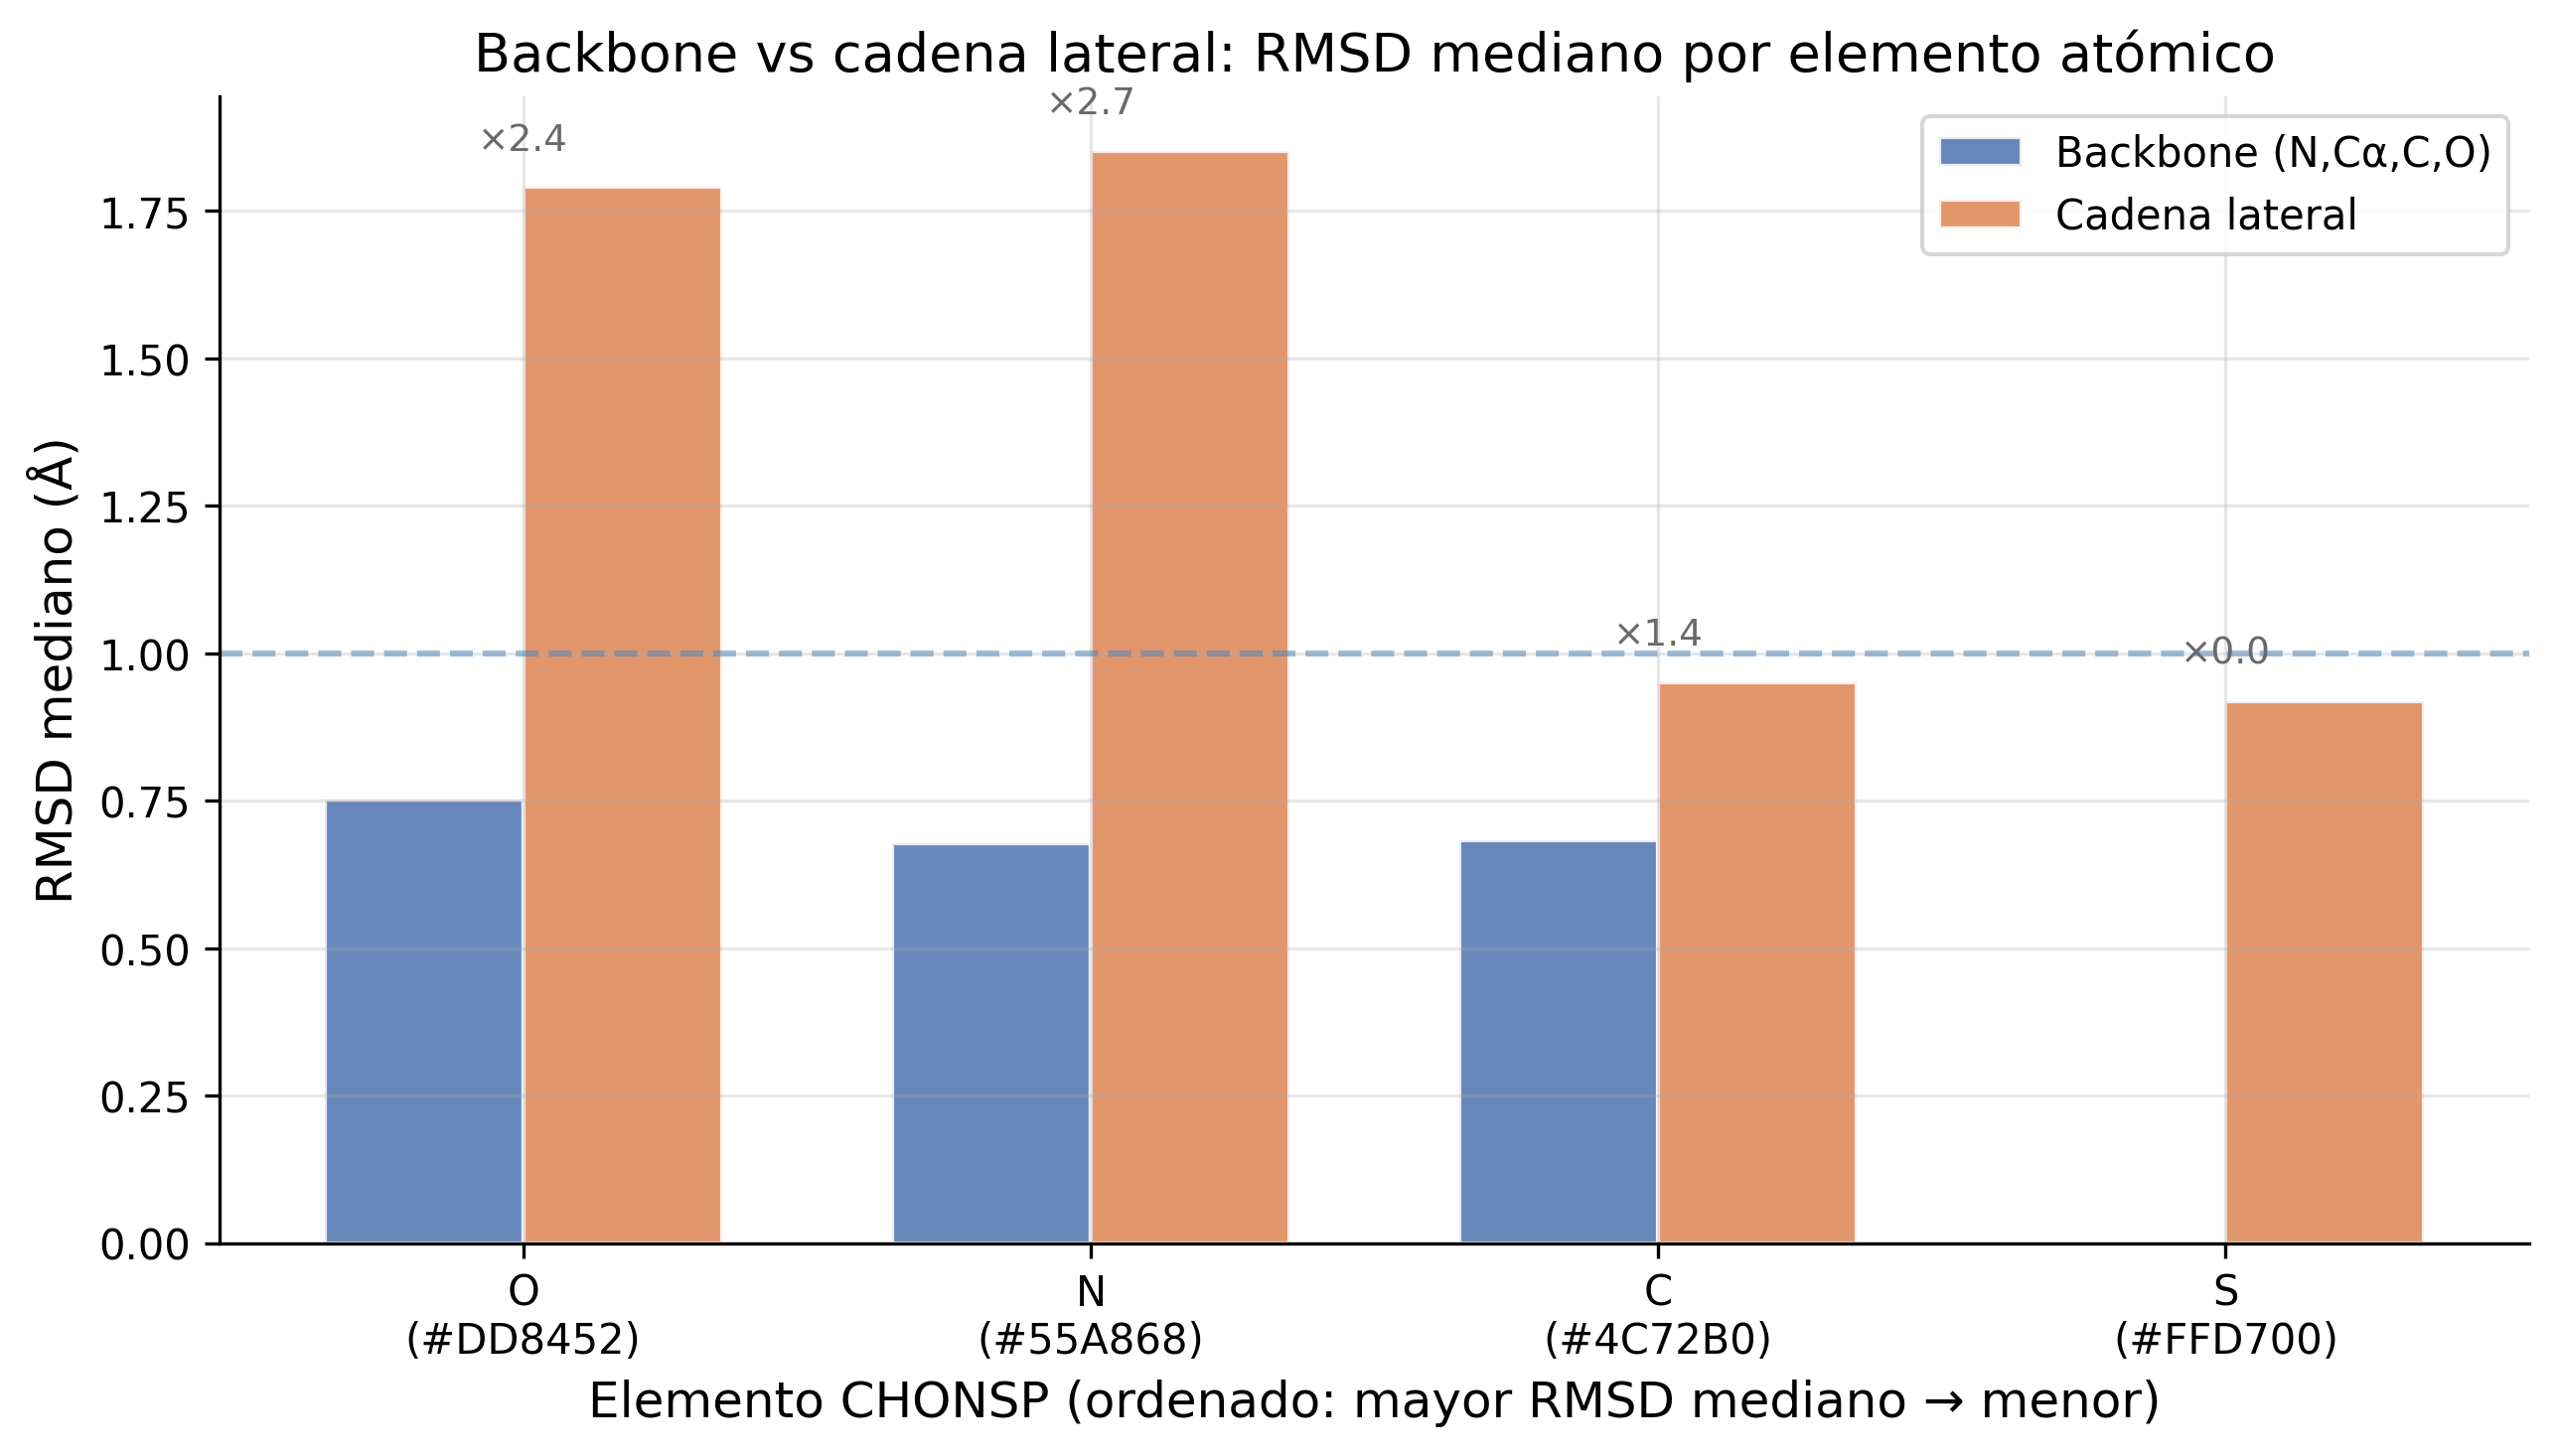
\includegraphics[width=0.76\linewidth]{atom_type_analysis.png}
        \\[-0.4em]
        {\scriptsize \textbf{Nivel 4:} \textit{Backbone} vs cadena lateral}
    \end{center}

    \vspace{-0.1em}
    \innerblock{\textbf{Gradiente de precisi\'on}}{
        \begin{itemize}[leftmargin=1em, itemsep=0em, topsep=0em]
            \item[\textcolor{itamblue}{$\blacktriangleright$}] \textbf{Mejor:}
                alif\'aticos del n\'ucleo (V, I, L)
            \item[\textcolor{itamaccent}{$\blacktriangleright$}] \textbf{Peor:}
                cargados de superficie (K, R, E)
            \item[\textcolor{itamblue}{$\blacktriangleright$}] \textit{Backbone} siempre
                m\'as preciso ($\times$1,1--1,4)
            \item[\textcolor{itamblue}{$\blacktriangleright$}] \textbf{C} $>$ \textbf{N}, \textbf{O}; \textbf{S} variable
        \end{itemize}
    }
}

\block{6. Inferencia bayesiana}{
    Modelo \textbf{Beta-Binomial}, prior $\text{Beta}(1,1)$,
    para $P(\text{RMSD} < 1\,\text{\AA})$:
    \vspace{-0.5em}
    \begin{equation*}
        p \mid k, n \;\sim\; \text{Beta}(1 + k,\; 1 + n - k)
    \end{equation*}
    \vspace{-0.7em}

    \begin{center}
        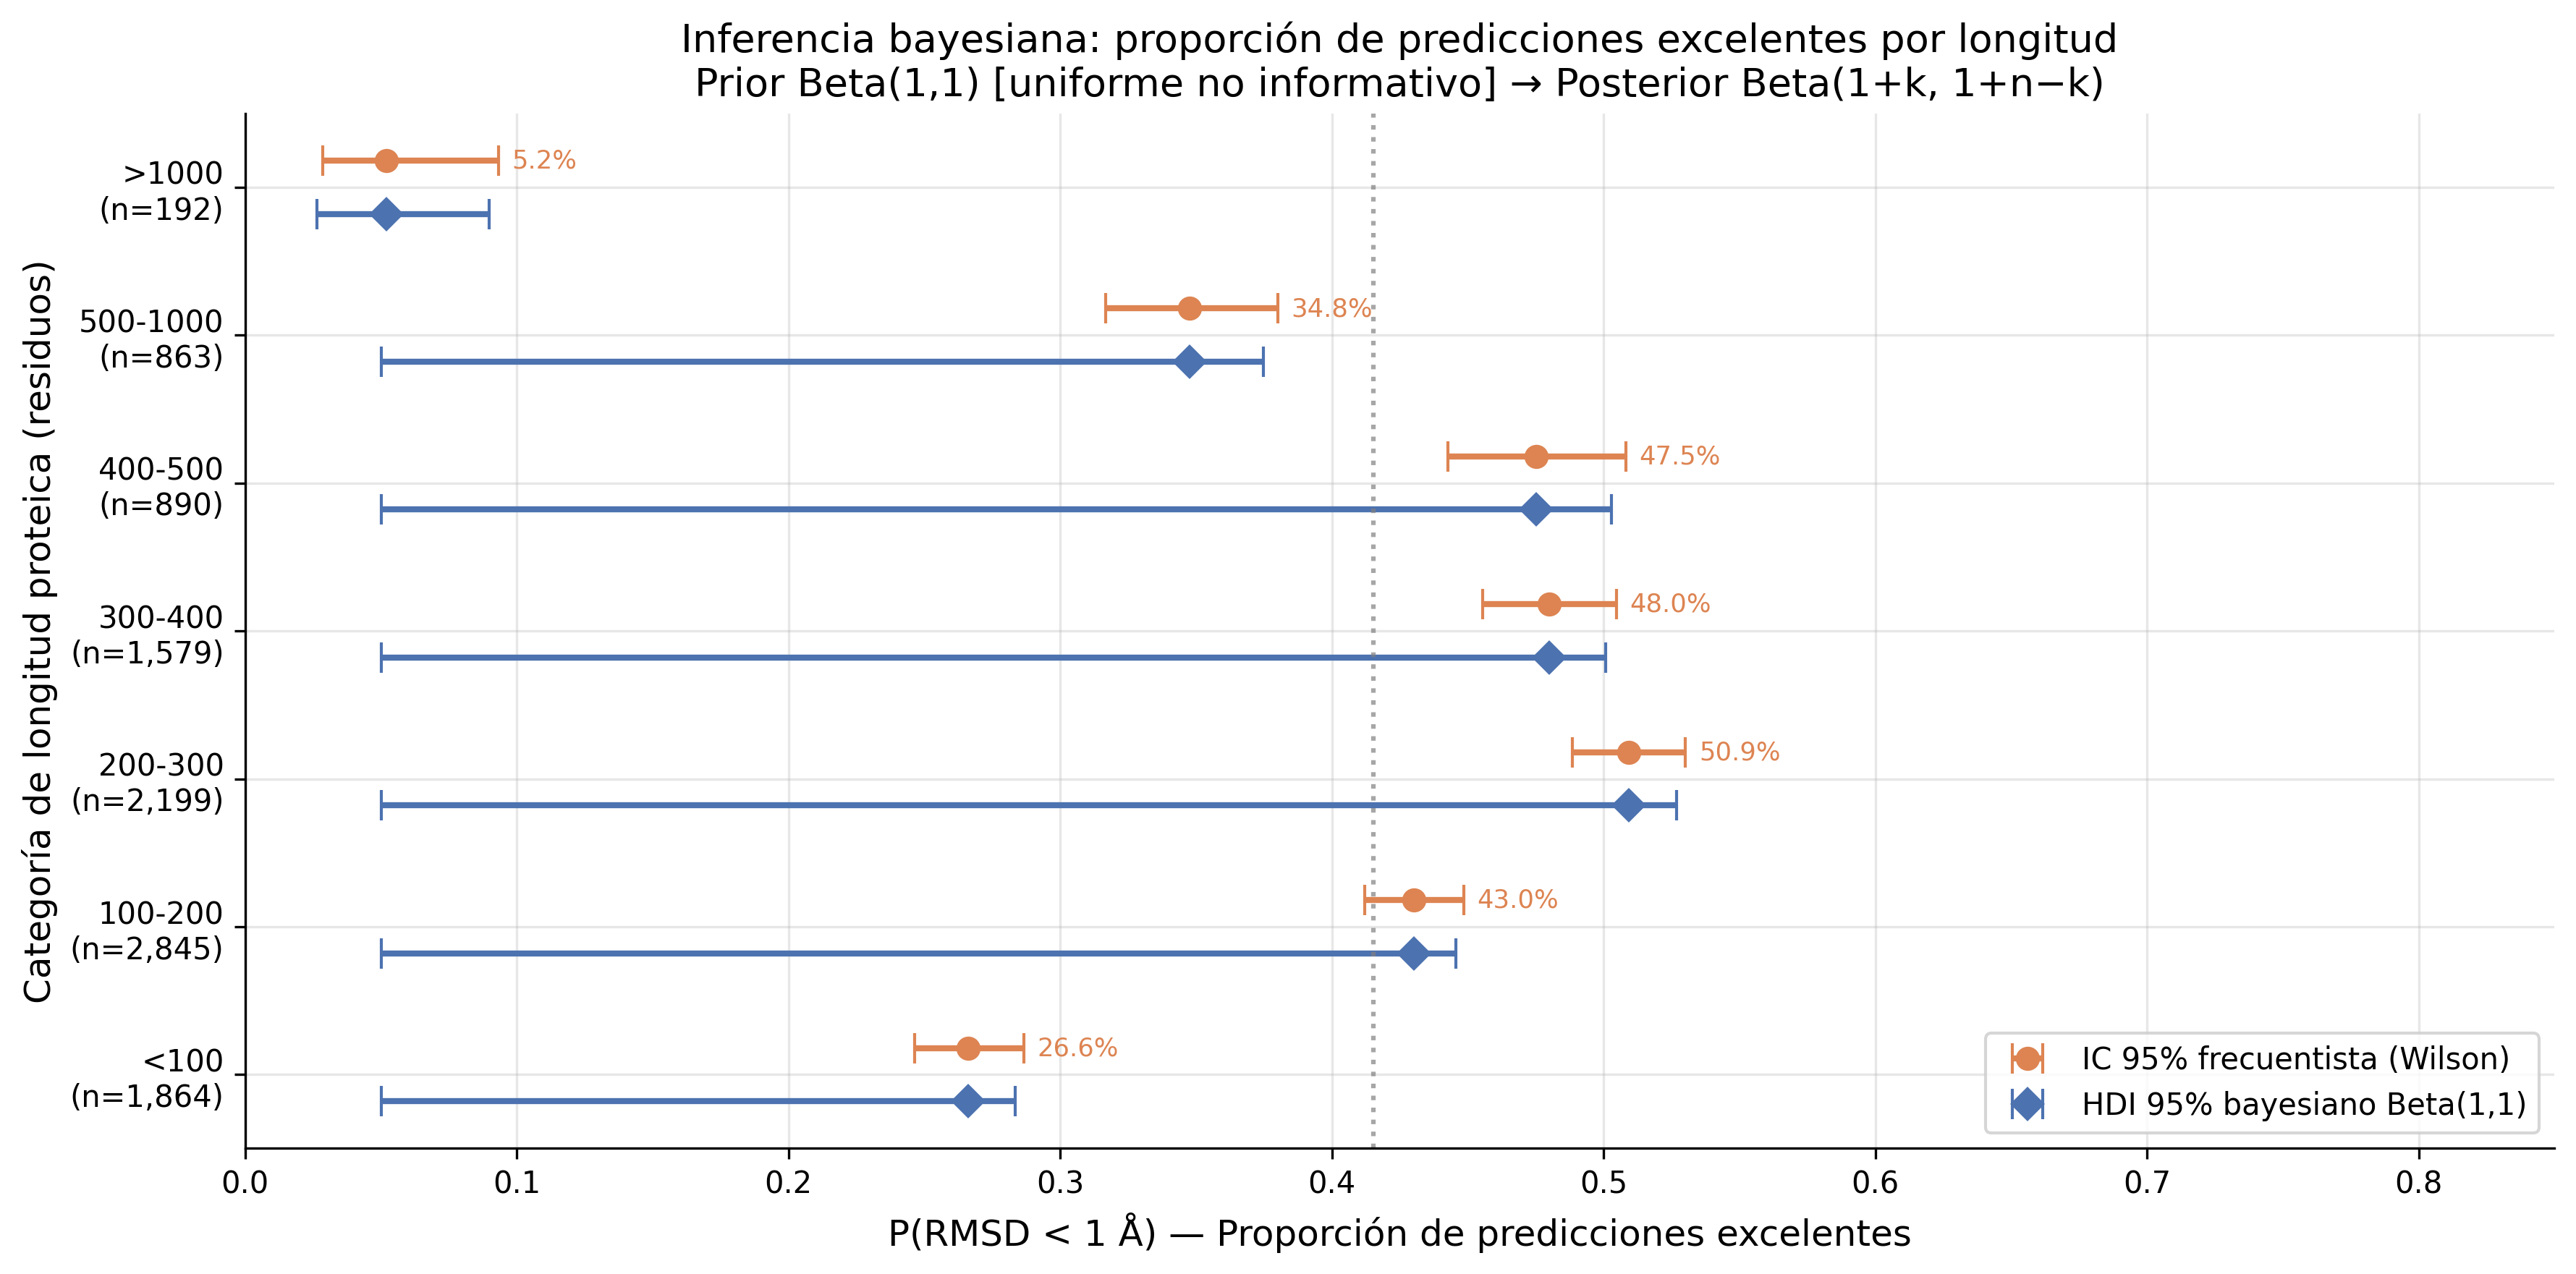
\includegraphics[width=0.95\linewidth]{fig_05_bayesian_ci.png}
        \\[-0.4em]
        {\scriptsize HDI 95\% bayesiano vs IC Wilson 95\%.}
    \end{center}

    \vspace{-0.1em}
    {\footnotesize Para $n$ grandes ambos convergen; en prote\'inas $>$1.000 res.
    la incertidumbre posterior aumenta por menor muestra.}
}

\block{Implicaciones biol\'ogicas}{
    \begin{itemize}
        \item Las regiones de \textbf{n\'ucleo hidrof\'obico} muestran mayor estabilidad
        geom\'etrica y menor dispersi\'on de RMSD.
        \item Residuos cargados de superficie concentran mayor error por movilidad,
        solvente y dependencia del entorno experimental.
        \item El \textit{backbone} es consistentemente m\'as confiable que cadenas laterales
        para an\'alisis comparativos de gran escala.
    \end{itemize}
}

\end{columns}

\block{7. Conclusiones cient\'ificas y recomendaciones}{
    \begin{minipage}[t]{0.31\linewidth}
        \innerblock{\textbf{Lectura principal}}{
            \begin{itemize}
                \item El mapeo SIFTS es obligatorio para comparaciones PDB--AlphaFold.
                \item La precisi\'on alta se concentra en 100--500 residuos.
                \item No hay ``\textit{sweet spot}'' real: era un artefacto de numeraci\'on.
            \end{itemize}
        }
    \end{minipage}%
    \hfill
    \begin{minipage}[t]{0.31\linewidth}
        \innerblock{\textbf{Uso recomendado}}{
            \begin{itemize}
                \item[\textcolor{itamblue}{$\checkmark$}] \textit{Docking} exploratorio y dise\~no de mutantes.
                \item[\textcolor{itamblue}{$\checkmark$}] Mayor confianza en n\'ucleo hidrof\'obico.
                \item[\textcolor{itamaccent}{$\triangle$}] Precauci\'on con estados \textit{holo}.
            \end{itemize}
        }
    \end{minipage}%
    \hfill
    \begin{minipage}[t]{0.31\linewidth}
        \innerblock{\textbf{Siguiente etapa}}{
            \begin{itemize}
                \item Evaluar AlphaFold3 bajo el mismo protocolo.
                \item Separar errores por dominio CATH/SCOP.
                \item Comparar con RoseTTAFold y ESMFold.
            \end{itemize}
        }
    \end{minipage}
}

\end{document}
